\chapter{Способ построения Актор-Критик САУ} \label{chapt2}

В подходе с обучением с подкреплением целью функционирования агента является максимизация целевой функции, который представляет собой суммарную величину награды - подкрепления. Такого типа управление относится к классу систем экстремального управления (СЭУ).

\section{Структурная схема системы экстремального управления} \label{sect2_1}
Системы экстремального управления относят к классу адаптивных систем, такие системы отличаются автоматическим выбором режима управления, при котором поддерживается минимальное или максимальное значение некой целевой функции. 

\begin{figure}[ht] 
  \center
  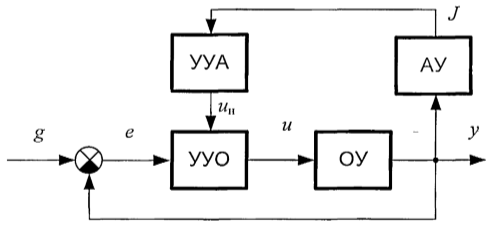
\includegraphics [scale=1] {seu_21}
  \caption{Структурная схема СЭУ} 
  \label{img:seu_21}  
\end{figure}



%\newpage
%============================================================================================================================
\section{Структурная схема Актор-Критик САУ} \label{sect2_2}
С помощью метода Актор-Критик и обучения с подкреплением разработана обобщенная структурная схема Актор-Критик САУ, изображенная на рисунке ~\ref{img:ac_struct}, а также алгоритмы функционирования системы
\begin{figure}[ht] 
	\center
	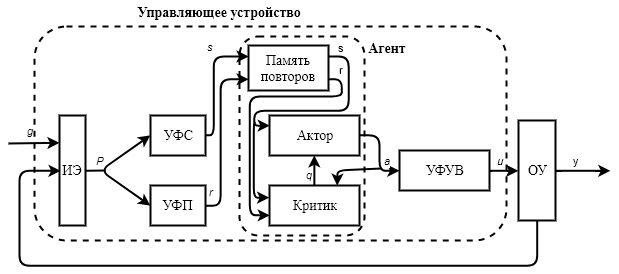
\includegraphics [scale=0.7] {ac_struct}
	\caption{Структурная схема Актор-Критик САУ} 
	\label{img:ac_struct}  
\end{figure}

Объект управления должен обладать свойствами частично наблюдаемого марковского процесса (POMDP)

\subsection{Импульсный элемент} \label{subsect2_2_1}
Целью функционирования импульсного элемента является дискретизация поступающего на вход сигнала с шагом $\tau_{\text{УУ}}$, который является параметром настройки УУ. ИЭ отвечает за формирование вектора дискретных сигналов $\bar{P}[k]$, который вектор поступает на входы УФС и УФП. Вектор $\bar{P}[k]$ состоит из $N_{\text{ОУ}}$ элементов, где $N_{\text{ОУ}}$ количество переменных состояния ОУ.

\subsection{Устройство формирования состояния} \label{subsect2_2_2}
Блок УФС отвечает за создание вектора состояний $s[k]$, который поступает на вход Актору и Критику. Данный вектор состоит из квантованных и нормализованных к масштабу [-1, 1] значений вектора $\bar{P}[k]$ 

\subsection{Устройство формирования подкрепления} \label{subsect2_2_3}

\subsection{Агент} \label{subsect2_2_4}
"Агент" является блоком, реализующим алгоритм, в основе функционирования которого лежит метод Актор-Критик. Данный метод был выбран на основе анализа, приведенного в главе \ref{subsect1_3_6}.

На вход данного блока подается вектор состояния $s[k]$ и сигнал подкрепления $r[k]$. Блок "Агент" состоит из двух подблоков: Актора и Критика. Актор отвечает за формирование сигнала управления и Критик за анализ качества управления. У "Агента" есть два режима функционирования:
\begin{enumerate}
	\item Обучение. Задействованы и Актор и Критик.
	\item Предсказание. Работает только Актор.
\end{enumerate} 

Параметрами настройки блока "Агент" являются:
\begin{itemize}
	\item $ N_s $ - количество состояний $s[k]$;
	\item $ N_a $ - количество параметров во множестве воздействий на ОУ $ A $;
	\item $ \gamma $ - коэффициент дисконтирования сигнала подкрепления;
	\item $ \Delta $ - коэффициент скорости обучения (learning rate);
	\item $ f_{\epsilon} $ - закон изменения коэффициента исследования;
	\item $ N_R $ - количество элементов в памяти повторов;
	\item также в качестве параметров настройки блока выступают количество слоев ИНС и количество нейронов в каждом из них.
\end{itemize}

\subsection{Устройство формирования управляющего воздействия} \label{subsect2_2_5}
Данное устройство предназначено за преобразование предсказанного "Агентом" действие в управляюее воздействие для конкретного ОУ.

